% Options for packages loaded elsewhere
\PassOptionsToPackage{unicode}{hyperref}
\PassOptionsToPackage{hyphens}{url}
\PassOptionsToPackage{dvipsnames,svgnames,x11names}{xcolor}
%
\documentclass[
  letterpaper,
  DIV=11,
  numbers=noendperiod]{scrreprt}

\usepackage{amsmath,amssymb}
\usepackage{lmodern}
\usepackage{iftex}
\ifPDFTeX
  \usepackage[T1]{fontenc}
  \usepackage[utf8]{inputenc}
  \usepackage{textcomp} % provide euro and other symbols
\else % if luatex or xetex
  \usepackage{unicode-math}
  \defaultfontfeatures{Scale=MatchLowercase}
  \defaultfontfeatures[\rmfamily]{Ligatures=TeX,Scale=1}
\fi
% Use upquote if available, for straight quotes in verbatim environments
\IfFileExists{upquote.sty}{\usepackage{upquote}}{}
\IfFileExists{microtype.sty}{% use microtype if available
  \usepackage[]{microtype}
  \UseMicrotypeSet[protrusion]{basicmath} % disable protrusion for tt fonts
}{}
\makeatletter
\@ifundefined{KOMAClassName}{% if non-KOMA class
  \IfFileExists{parskip.sty}{%
    \usepackage{parskip}
  }{% else
    \setlength{\parindent}{0pt}
    \setlength{\parskip}{6pt plus 2pt minus 1pt}}
}{% if KOMA class
  \KOMAoptions{parskip=half}}
\makeatother
\usepackage{xcolor}
\setlength{\emergencystretch}{3em} % prevent overfull lines
\setcounter{secnumdepth}{5}
% Make \paragraph and \subparagraph free-standing
\ifx\paragraph\undefined\else
  \let\oldparagraph\paragraph
  \renewcommand{\paragraph}[1]{\oldparagraph{#1}\mbox{}}
\fi
\ifx\subparagraph\undefined\else
  \let\oldsubparagraph\subparagraph
  \renewcommand{\subparagraph}[1]{\oldsubparagraph{#1}\mbox{}}
\fi

\usepackage{color}
\usepackage{fancyvrb}
\newcommand{\VerbBar}{|}
\newcommand{\VERB}{\Verb[commandchars=\\\{\}]}
\DefineVerbatimEnvironment{Highlighting}{Verbatim}{commandchars=\\\{\}}
% Add ',fontsize=\small' for more characters per line
\usepackage{framed}
\definecolor{shadecolor}{RGB}{241,243,245}
\newenvironment{Shaded}{\begin{snugshade}}{\end{snugshade}}
\newcommand{\AlertTok}[1]{\textcolor[rgb]{0.68,0.00,0.00}{#1}}
\newcommand{\AnnotationTok}[1]{\textcolor[rgb]{0.37,0.37,0.37}{#1}}
\newcommand{\AttributeTok}[1]{\textcolor[rgb]{0.40,0.45,0.13}{#1}}
\newcommand{\BaseNTok}[1]{\textcolor[rgb]{0.68,0.00,0.00}{#1}}
\newcommand{\BuiltInTok}[1]{\textcolor[rgb]{0.00,0.23,0.31}{#1}}
\newcommand{\CharTok}[1]{\textcolor[rgb]{0.13,0.47,0.30}{#1}}
\newcommand{\CommentTok}[1]{\textcolor[rgb]{0.37,0.37,0.37}{#1}}
\newcommand{\CommentVarTok}[1]{\textcolor[rgb]{0.37,0.37,0.37}{\textit{#1}}}
\newcommand{\ConstantTok}[1]{\textcolor[rgb]{0.56,0.35,0.01}{#1}}
\newcommand{\ControlFlowTok}[1]{\textcolor[rgb]{0.00,0.23,0.31}{#1}}
\newcommand{\DataTypeTok}[1]{\textcolor[rgb]{0.68,0.00,0.00}{#1}}
\newcommand{\DecValTok}[1]{\textcolor[rgb]{0.68,0.00,0.00}{#1}}
\newcommand{\DocumentationTok}[1]{\textcolor[rgb]{0.37,0.37,0.37}{\textit{#1}}}
\newcommand{\ErrorTok}[1]{\textcolor[rgb]{0.68,0.00,0.00}{#1}}
\newcommand{\ExtensionTok}[1]{\textcolor[rgb]{0.00,0.23,0.31}{#1}}
\newcommand{\FloatTok}[1]{\textcolor[rgb]{0.68,0.00,0.00}{#1}}
\newcommand{\FunctionTok}[1]{\textcolor[rgb]{0.28,0.35,0.67}{#1}}
\newcommand{\ImportTok}[1]{\textcolor[rgb]{0.00,0.46,0.62}{#1}}
\newcommand{\InformationTok}[1]{\textcolor[rgb]{0.37,0.37,0.37}{#1}}
\newcommand{\KeywordTok}[1]{\textcolor[rgb]{0.00,0.23,0.31}{#1}}
\newcommand{\NormalTok}[1]{\textcolor[rgb]{0.00,0.23,0.31}{#1}}
\newcommand{\OperatorTok}[1]{\textcolor[rgb]{0.37,0.37,0.37}{#1}}
\newcommand{\OtherTok}[1]{\textcolor[rgb]{0.00,0.23,0.31}{#1}}
\newcommand{\PreprocessorTok}[1]{\textcolor[rgb]{0.68,0.00,0.00}{#1}}
\newcommand{\RegionMarkerTok}[1]{\textcolor[rgb]{0.00,0.23,0.31}{#1}}
\newcommand{\SpecialCharTok}[1]{\textcolor[rgb]{0.37,0.37,0.37}{#1}}
\newcommand{\SpecialStringTok}[1]{\textcolor[rgb]{0.13,0.47,0.30}{#1}}
\newcommand{\StringTok}[1]{\textcolor[rgb]{0.13,0.47,0.30}{#1}}
\newcommand{\VariableTok}[1]{\textcolor[rgb]{0.07,0.07,0.07}{#1}}
\newcommand{\VerbatimStringTok}[1]{\textcolor[rgb]{0.13,0.47,0.30}{#1}}
\newcommand{\WarningTok}[1]{\textcolor[rgb]{0.37,0.37,0.37}{\textit{#1}}}

\providecommand{\tightlist}{%
  \setlength{\itemsep}{0pt}\setlength{\parskip}{0pt}}\usepackage{longtable,booktabs,array}
\usepackage{calc} % for calculating minipage widths
% Correct order of tables after \paragraph or \subparagraph
\usepackage{etoolbox}
\makeatletter
\patchcmd\longtable{\par}{\if@noskipsec\mbox{}\fi\par}{}{}
\makeatother
% Allow footnotes in longtable head/foot
\IfFileExists{footnotehyper.sty}{\usepackage{footnotehyper}}{\usepackage{footnote}}
\makesavenoteenv{longtable}
\usepackage{graphicx}
\makeatletter
\def\maxwidth{\ifdim\Gin@nat@width>\linewidth\linewidth\else\Gin@nat@width\fi}
\def\maxheight{\ifdim\Gin@nat@height>\textheight\textheight\else\Gin@nat@height\fi}
\makeatother
% Scale images if necessary, so that they will not overflow the page
% margins by default, and it is still possible to overwrite the defaults
% using explicit options in \includegraphics[width, height, ...]{}
\setkeys{Gin}{width=\maxwidth,height=\maxheight,keepaspectratio}
% Set default figure placement to htbp
\makeatletter
\def\fps@figure{htbp}
\makeatother

\KOMAoption{captions}{tableheading}
\makeatletter
\makeatother
\makeatletter
\@ifpackageloaded{bookmark}{}{\usepackage{bookmark}}
\makeatother
\makeatletter
\@ifpackageloaded{caption}{}{\usepackage{caption}}
\AtBeginDocument{%
\ifdefined\contentsname
  \renewcommand*\contentsname{Table of contents}
\else
  \newcommand\contentsname{Table of contents}
\fi
\ifdefined\listfigurename
  \renewcommand*\listfigurename{List of Figures}
\else
  \newcommand\listfigurename{List of Figures}
\fi
\ifdefined\listtablename
  \renewcommand*\listtablename{List of Tables}
\else
  \newcommand\listtablename{List of Tables}
\fi
\ifdefined\figurename
  \renewcommand*\figurename{Figure}
\else
  \newcommand\figurename{Figure}
\fi
\ifdefined\tablename
  \renewcommand*\tablename{Table}
\else
  \newcommand\tablename{Table}
\fi
}
\@ifpackageloaded{float}{}{\usepackage{float}}
\floatstyle{ruled}
\@ifundefined{c@chapter}{\newfloat{codelisting}{h}{lop}}{\newfloat{codelisting}{h}{lop}[chapter]}
\floatname{codelisting}{Listing}
\newcommand*\listoflistings{\listof{codelisting}{List of Listings}}
\makeatother
\makeatletter
\@ifpackageloaded{caption}{}{\usepackage{caption}}
\@ifpackageloaded{subcaption}{}{\usepackage{subcaption}}
\makeatother
\makeatletter
\@ifpackageloaded{tcolorbox}{}{\usepackage[many]{tcolorbox}}
\makeatother
\makeatletter
\@ifundefined{shadecolor}{\definecolor{shadecolor}{rgb}{.97, .97, .97}}
\makeatother
\makeatletter
\makeatother
\ifLuaTeX
  \usepackage{selnolig}  % disable illegal ligatures
\fi
\IfFileExists{bookmark.sty}{\usepackage{bookmark}}{\usepackage{hyperref}}
\IfFileExists{xurl.sty}{\usepackage{xurl}}{} % add URL line breaks if available
\urlstyle{same} % disable monospaced font for URLs
\hypersetup{
  pdftitle={Peace and Trust Progress Journal},
  colorlinks=true,
  linkcolor={blue},
  filecolor={Maroon},
  citecolor={Blue},
  urlcolor={Blue},
  pdfcreator={LaTeX via pandoc}}

\title{Peace and Trust Progress Journal}
\author{}
\date{}

\begin{document}
\maketitle
\ifdefined\Shaded\renewenvironment{Shaded}{\begin{tcolorbox}[frame hidden, enhanced, sharp corners, borderline west={3pt}{0pt}{shadecolor}, boxrule=0pt, interior hidden, breakable]}{\end{tcolorbox}}\fi

\renewcommand*\contentsname{Table of contents}
{
\hypersetup{linkcolor=}
\setcounter{tocdepth}{2}
\tableofcontents
}
\bookmarksetup{startatroot}

\hypertarget{introduction}{%
\chapter*{Introduction}\label{introduction}}
\addcontentsline{toc}{chapter}{Introduction}

This progress journal covers PEACE AND TRUST's work during their term at
\href{https://mef-bda503.github.io/fall22/}{BDA 503 Fall 2022}.

Each section is an assignment or an individual work.

\bookmarksetup{startatroot}

\hypertarget{startups-2021}{%
\chapter{STARTUPS 2021}\label{startups-2021}}

In this report, we will explore the data set of start-ups getting
investments from a variety of domestic and international investors. Data
is gathered from \textbf{KPMG} and \textbf{212}'s
\href{https://assets.kpmg/content/dam/kpmg/tr/pdf/2022/03/turkish-startup-investments-review-2021.pdf}{Turkish
Startup Investments Review 2021 report}.

\begin{enumerate}
\def\labelenumi{\arabic{enumi}.}
\tightlist
\item
  In the seed stage, gaming sector has the lead, in the acquistion
  sector, SaaS is the leader sector
\item
  Gaming is winner of number of investment category, but if we look at
  total deals Ecommerce Enabler sector is winner. This is possibly due
  to the trendyol,hepsiburada investments which are outliers of this
  category. Delivery \& Logistic sector is also ahead of Gaming, this is
  also due to the getir, which is also a outlier in terms of deal
  amount.
\item
  Gaming sector has the highest number of investors
\item
  Agritech sector is the most multi-cultural sector in terms of
  different number of investor origins in one deal
\item
  Most of the investments made in December and August, and the most
  quite months are May and October, as quarters, number of total
  investments are increasing in Q3,Q4 if we compare Q1 and Q2.
\item
  Fintech startups' 73\% of investments coming from Financial Investors.
  Interestingly, 86\% of Delivery \& Logistics investments and 78\% of
  Healthtech investments coming from Financial Investors which are
  greater than Fintech.
\end{enumerate}

\hypertarget{data-preprocessing}{%
\subsection{DATA PREPROCESSING}\label{data-preprocessing}}

Install necessary packages

\begin{Shaded}
\begin{Highlighting}[]
\FunctionTok{install.packages}\NormalTok{(}\StringTok{"readxl"}\NormalTok{)}
\end{Highlighting}
\end{Shaded}

Call necessary libraries

\begin{Shaded}
\begin{Highlighting}[]
\FunctionTok{library}\NormalTok{(readxl)}
\FunctionTok{library}\NormalTok{(lubridate)}
\FunctionTok{library}\NormalTok{(dplyr)}
\FunctionTok{library}\NormalTok{(tidyverse)}
\FunctionTok{library}\NormalTok{(ggplot2)}
\end{Highlighting}
\end{Shaded}

Load the data

\begin{Shaded}
\begin{Highlighting}[]
\NormalTok{data }\OtherTok{=} \FunctionTok{read\_excel}\NormalTok{(}\StringTok{"data//startup\_deals\_2021.xlsx"}\NormalTok{)}
\end{Highlighting}
\end{Shaded}

Rename the column names

\begin{Shaded}
\begin{Highlighting}[]
\NormalTok{data }\OtherTok{\textless{}{-}}\NormalTok{ data }\SpecialCharTok{\%\textgreater{}\%} 
  \FunctionTok{rename}\NormalTok{(}\AttributeTok{Stage =} \StringTok{\textquotesingle{}Investment Stage\textquotesingle{}}\NormalTok{,}
         \AttributeTok{Company =} \StringTok{\textquotesingle{}Target Company\textquotesingle{}}\NormalTok{,}
         \AttributeTok{DealValue =} \StringTok{\textquotesingle{}Deal Value (USD)\textquotesingle{}}\NormalTok{,}
         \AttributeTok{Financial =} \StringTok{\textquotesingle{}Financial Investor\textquotesingle{}}\NormalTok{,}
         \AttributeTok{Date =} \StringTok{\textquotesingle{}Announcement Date\textquotesingle{}}\NormalTok{,}
         \AttributeTok{Origin =}\StringTok{"Investor\textquotesingle{}s Origin"}\NormalTok{,}
         \AttributeTok{Stake =} \StringTok{"Stake (\%)"}
\NormalTok{  )}
\FunctionTok{colnames}\NormalTok{(data)}
\end{Highlighting}
\end{Shaded}

\begin{verbatim}
[1] "Company"   "Sector"    "Investor"  "Date"      "Financial" "Origin"   
[7] "Stake"     "DealValue" "Stage"    
\end{verbatim}

\begin{itemize}
\tightlist
\item
  Convert ``Deal Value (USD)'' type to numeric data
\item
  Convert Date column to date type, and drop year 2021, since all date
  values have same year, 2021
\item
  Drop \% sign for Stake, and convert to numeric data type
\end{itemize}

\begin{Shaded}
\begin{Highlighting}[]
\FunctionTok{options}\NormalTok{(}\AttributeTok{scipen=}\DecValTok{999}\NormalTok{)}
\NormalTok{data}\SpecialCharTok{$}\NormalTok{DealValue }\OtherTok{\textless{}{-}} \FunctionTok{suppressWarnings}\NormalTok{(}\FunctionTok{as.numeric}\NormalTok{(data}\SpecialCharTok{$}\NormalTok{DealValue))}

\NormalTok{data}\SpecialCharTok{$}\NormalTok{Date }\OtherTok{\textless{}{-}} \FunctionTok{my}\NormalTok{(data}\SpecialCharTok{$}\NormalTok{Date)}


\NormalTok{data }\OtherTok{\textless{}{-}}\NormalTok{ data }\SpecialCharTok{\%\textgreater{}\%} 
  \FunctionTok{mutate}\NormalTok{(}\AttributeTok{Stake =} \FunctionTok{str\_replace\_all}\NormalTok{(Stake, }\StringTok{"\%"}\NormalTok{, }\StringTok{""}\NormalTok{))}
\NormalTok{data}\SpecialCharTok{$}\NormalTok{Stake }\OtherTok{\textless{}{-}} \FunctionTok{suppressWarnings}\NormalTok{(}\FunctionTok{as.numeric}\NormalTok{(data}\SpecialCharTok{$}\NormalTok{Stake))}
\FunctionTok{sapply}\NormalTok{(data, class)}
\end{Highlighting}
\end{Shaded}

\begin{verbatim}
    Company      Sector    Investor        Date   Financial      Origin 
"character" "character" "character"      "Date" "character" "character" 
      Stake   DealValue       Stage 
  "numeric"   "numeric" "character" 
\end{verbatim}

Sector feature has inconsistent values like Diğital Comparison,
Artificial intelligence, Cybersec urity, Telecpm, Artificial
Intelligence, B lockchain.

\begin{Shaded}
\begin{Highlighting}[]
\NormalTok{data\_incons }\OtherTok{\textless{}{-}}\NormalTok{ data }\SpecialCharTok{\%\textgreater{}\%}
  \FunctionTok{filter}\NormalTok{(Sector }\SpecialCharTok{\%in\%} \FunctionTok{c}\NormalTok{(}\StringTok{\textquotesingle{}Diğital Comparison\textquotesingle{}}\NormalTok{,}
\StringTok{\textquotesingle{}Artificial intelligence\textquotesingle{}}\NormalTok{,}
\StringTok{\textquotesingle{}Cybersec urity\textquotesingle{}}\NormalTok{,}
\StringTok{\textquotesingle{}Telecpm\textquotesingle{}}\NormalTok{,}
\StringTok{\textquotesingle{}Artificial Intelligence\textquotesingle{}}\NormalTok{,}
\StringTok{\textquotesingle{}B lockchain\textquotesingle{}}
\NormalTok{))}
\FunctionTok{unique}\NormalTok{(data\_incons}\SpecialCharTok{$}\NormalTok{Sector)}
\end{Highlighting}
\end{Shaded}

\begin{verbatim}
[1] "Artificial Intelligence" "Artificial intelligence"
[3] "B lockchain"             "Diğital Comparison"     
[5] "Cybersec urity"          "Telecpm"                
\end{verbatim}

Inconsistent Sector values are updated with the right values.

\begin{Shaded}
\begin{Highlighting}[]
\NormalTok{data}\SpecialCharTok{$}\NormalTok{Sector[data}\SpecialCharTok{$}\NormalTok{Sector }\SpecialCharTok{==} \StringTok{\textquotesingle{}Artificial intelligence\textquotesingle{}}\NormalTok{] }\OtherTok{\textless{}{-}} \StringTok{\textquotesingle{}Artificial Intelligence\textquotesingle{}}
\NormalTok{data}\SpecialCharTok{$}\NormalTok{Sector[data}\SpecialCharTok{$}\NormalTok{Sector }\SpecialCharTok{==} \StringTok{\textquotesingle{}Telecpm\textquotesingle{}}\NormalTok{] }\OtherTok{\textless{}{-}} \StringTok{\textquotesingle{}Telecom\textquotesingle{}}
\NormalTok{data}\SpecialCharTok{$}\NormalTok{Sector[data}\SpecialCharTok{$}\NormalTok{Sector }\SpecialCharTok{==} \StringTok{\textquotesingle{}B lockchain\textquotesingle{}}\NormalTok{] }\OtherTok{\textless{}{-}} \StringTok{\textquotesingle{}Blockchain\textquotesingle{}}
\NormalTok{data}\SpecialCharTok{$}\NormalTok{Sector[data}\SpecialCharTok{$}\NormalTok{Sector }\SpecialCharTok{==} \StringTok{\textquotesingle{}Diğital \textquotesingle{}}\NormalTok{] }\OtherTok{\textless{}{-}} \StringTok{\textquotesingle{}Dijital\textquotesingle{}}
\NormalTok{data}\SpecialCharTok{$}\NormalTok{Sector[data}\SpecialCharTok{$}\NormalTok{Sector }\SpecialCharTok{==} \StringTok{\textquotesingle{}Cybersec urity \textquotesingle{}}\NormalTok{] }\OtherTok{\textless{}{-}} \StringTok{\textquotesingle{}Cybersecurity\textquotesingle{}}
\NormalTok{data}\SpecialCharTok{$}\NormalTok{Sector[data}\SpecialCharTok{$}\NormalTok{Sector }\SpecialCharTok{==} \StringTok{\textquotesingle{}Ecommerce enabler\textquotesingle{}}\NormalTok{] }\OtherTok{\textless{}{-}} \StringTok{\textquotesingle{}Ecommerce Enabler\textquotesingle{}}
\NormalTok{data}\SpecialCharTok{$}\NormalTok{sector[data}\SpecialCharTok{$}\NormalTok{Sector }\SpecialCharTok{==} \StringTok{\textquotesingle{}I mage process\textquotesingle{}}\NormalTok{] }\OtherTok{\textless{}{-}} \StringTok{\textquotesingle{}Image process\textquotesingle{}}
\end{Highlighting}
\end{Shaded}

Now the data is ready for the EDA,

\begin{Shaded}
\begin{Highlighting}[]
\NormalTok{knitr}\SpecialCharTok{::}\FunctionTok{kable}\NormalTok{(}\FunctionTok{head}\NormalTok{(data))}
\end{Highlighting}
\end{Shaded}

\begin{longtable}[]{@{}
  >{\raggedright\arraybackslash}p{(\columnwidth - 18\tabcolsep) * \real{0.0652}}
  >{\raggedright\arraybackslash}p{(\columnwidth - 18\tabcolsep) * \real{0.1033}}
  >{\raggedright\arraybackslash}p{(\columnwidth - 18\tabcolsep) * \real{0.4674}}
  >{\raggedright\arraybackslash}p{(\columnwidth - 18\tabcolsep) * \real{0.0598}}
  >{\raggedright\arraybackslash}p{(\columnwidth - 18\tabcolsep) * \real{0.0543}}
  >{\raggedright\arraybackslash}p{(\columnwidth - 18\tabcolsep) * \real{0.0652}}
  >{\raggedleft\arraybackslash}p{(\columnwidth - 18\tabcolsep) * \real{0.0326}}
  >{\raggedleft\arraybackslash}p{(\columnwidth - 18\tabcolsep) * \real{0.0543}}
  >{\raggedright\arraybackslash}p{(\columnwidth - 18\tabcolsep) * \real{0.0598}}
  >{\raggedright\arraybackslash}p{(\columnwidth - 18\tabcolsep) * \real{0.0380}}@{}}
\toprule()
\begin{minipage}[b]{\linewidth}\raggedright
Company
\end{minipage} & \begin{minipage}[b]{\linewidth}\raggedright
Sector
\end{minipage} & \begin{minipage}[b]{\linewidth}\raggedright
Investor
\end{minipage} & \begin{minipage}[b]{\linewidth}\raggedright
Date
\end{minipage} & \begin{minipage}[b]{\linewidth}\raggedright
Financial
\end{minipage} & \begin{minipage}[b]{\linewidth}\raggedright
Origin
\end{minipage} & \begin{minipage}[b]{\linewidth}\raggedleft
Stake
\end{minipage} & \begin{minipage}[b]{\linewidth}\raggedleft
DealValue
\end{minipage} & \begin{minipage}[b]{\linewidth}\raggedright
Stage
\end{minipage} & \begin{minipage}[b]{\linewidth}\raggedright
sector
\end{minipage} \\
\midrule()
\endhead
Abonesepeti & SaaS & Keiretsu Forum, Berkan Burla & 2021-06-01 & Yes &
Turkey & 5 & 100000 & Seed Stage & NA \\
Abrakadabra & Gaming & WePlay Ventures & 2021-12-01 & Yes & Turkey & 5 &
250000 & Seed Stage & NA \\
Ace Games & Gaming & Actera Group, NFX, Kristian Segerstrale, Alexis
Bonte, Kaan Günay (Private Investors) & 2021-04-01 & Yes & Turkey, USA &
NA & NA & Seed Stage & NA \\
Adlema & Internet of things & TR Angels & 2021-06-01 & Yes & Turkey & NA
& 120000 & Seed Stage & NA \\
Agave Games & Gaming & 500 Istanbul (Fund II), Akin Babayiğit (Private
Investor) & 2021-09-01 & Yes & Turkey & NA & 100000 & Seed Stage & NA \\
Agrio & Fintech & lnnovate21st.com & 2021-06-01 & Yes & Turkey & NA &
1000000 & Seed Stage & NA \\
\bottomrule()
\end{longtable}

\hypertarget{exploratory-data-analysis}{%
\subsection{EXPLORATORY DATA ANALYSIS}\label{exploratory-data-analysis}}

\hypertarget{first-3-sectors-of-each-stage-gaming-is-a-good-start}{%
\subsubsection{First 3 Sectors of each Stage: Gaming is a good
start!}\label{first-3-sectors-of-each-stage-gaming-is-a-good-start}}

\begin{Shaded}
\begin{Highlighting}[]
\NormalTok{sector\_stage }\OtherTok{\textless{}{-}}\NormalTok{ data }\SpecialCharTok{\%\textgreater{}\%}
  \FunctionTok{group\_by}\NormalTok{(Stage,Sector) }\SpecialCharTok{\%\textgreater{}\%}
  \FunctionTok{summarise}\NormalTok{(}\AttributeTok{Total =} \FunctionTok{n}\NormalTok{()) }\SpecialCharTok{\%\textgreater{}\%} 
  \FunctionTok{arrange}\NormalTok{(}\FunctionTok{desc}\NormalTok{(Total)) }\SpecialCharTok{\%\textgreater{}\%}
  \FunctionTok{slice\_max}\NormalTok{(Total,}\AttributeTok{n=}\DecValTok{3}\NormalTok{)}
\NormalTok{knitr}\SpecialCharTok{::}\FunctionTok{kable}\NormalTok{(sector\_stage)}
\end{Highlighting}
\end{Shaded}

\begin{longtable}[]{@{}llr@{}}
\toprule()
Stage & Sector & Total \\
\midrule()
\endhead
Acquisition & SaaS & 10 \\
Acquisition & Gaming & 5 \\
Acquisition & Fintech & 4 \\
Early VC Stage & Fintech & 3 \\
Early VC Stage & Ecommerce Enabler & 2 \\
Early VC Stage & Foodtech & 2 \\
Early VC Stage & Gaming & 2 \\
Later VC Stage & Delivery \& Logistics & 3 \\
Seed Stage & Gaming & 44 \\
Seed Stage & SaaS & 17 \\
Seed Stage & Fintech & 16 \\
\bottomrule()
\end{longtable}

\begin{Shaded}
\begin{Highlighting}[]
\FunctionTok{ggplot}\NormalTok{(}\AttributeTok{data=}\NormalTok{sector\_stage, }\FunctionTok{aes}\NormalTok{(}\AttributeTok{x=}\NormalTok{Stage, }\AttributeTok{y=}\NormalTok{Total, }\AttributeTok{fill=}\FunctionTok{factor}\NormalTok{(Sector))) }\SpecialCharTok{+}
  \FunctionTok{geom\_bar}\NormalTok{(}\AttributeTok{position=}\StringTok{"dodge"}\NormalTok{,}\AttributeTok{stat=}\StringTok{"identity"}\NormalTok{) }\SpecialCharTok{+} 
  \FunctionTok{ggtitle}\NormalTok{(}\StringTok{"Investment Stage and Investment Sectors"}\NormalTok{)}
\end{Highlighting}
\end{Shaded}

\begin{figure}[H]

{\centering 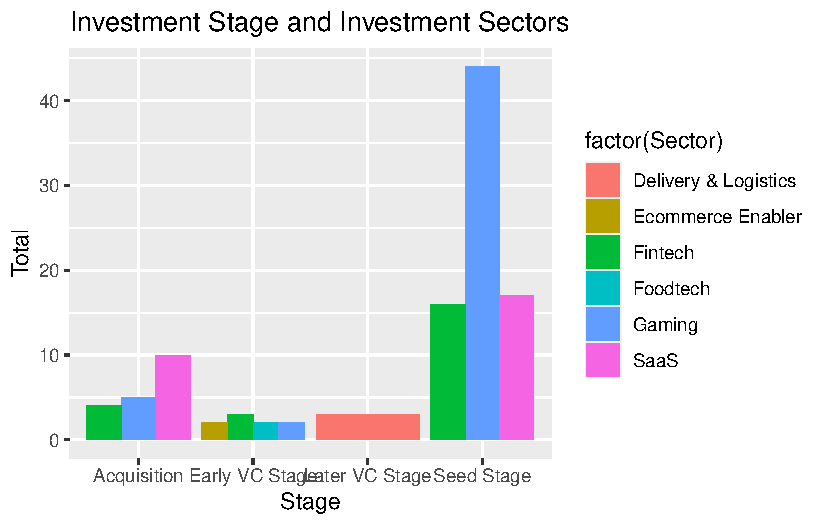
\includegraphics{./assignment1_files/figure-pdf/unnamed-chunk-3-1.pdf}

}

\end{figure}

\hypertarget{deal-amounts-a-general-look}{%
\subsubsection{Deal Amounts: A General
Look}\label{deal-amounts-a-general-look}}

\begin{Shaded}
\begin{Highlighting}[]
\NormalTok{df1 }\OtherTok{\textless{}{-}}\NormalTok{  data }\SpecialCharTok{\%\textgreater{}\%}
  \FunctionTok{mutate}\NormalTok{(}\AttributeTok{TotalDeal =} \FunctionTok{sum}\NormalTok{(DealValue,}\AttributeTok{na.rm =} \ConstantTok{TRUE}\NormalTok{))}

 
\NormalTok{df2 }\OtherTok{\textless{}{-}}\NormalTok{ df1 }\SpecialCharTok{\%\textgreater{}\%}
  \FunctionTok{group\_by}\NormalTok{(Sector) }\SpecialCharTok{\%\textgreater{}\%}
  \FunctionTok{summarise}\NormalTok{(}\AttributeTok{RateOfDeal=}\NormalTok{(}\FunctionTok{sum}\NormalTok{(DealValue,}\AttributeTok{na.rm =} \ConstantTok{TRUE}\NormalTok{)}\SpecialCharTok{/}\NormalTok{TotalDeal)}\SpecialCharTok{*}\DecValTok{100}\NormalTok{) }\SpecialCharTok{\%\textgreater{}\%}
  \FunctionTok{arrange}\NormalTok{(}\FunctionTok{desc}\NormalTok{(RateOfDeal)) }
  

\NormalTok{knitr}\SpecialCharTok{::}\FunctionTok{kable}\NormalTok{(}\FunctionTok{head}\NormalTok{(}\FunctionTok{unique}\NormalTok{(df2)))}
\end{Highlighting}
\end{Shaded}

\begin{longtable}[]{@{}lr@{}}
\toprule()
Sector & RateOfDeal \\
\midrule()
\endhead
Ecommerce Enabler & 58.7822478 \\
Delivery \& Logistics & 27.1997590 \\
Gaming & 5.8547176 \\
SaaS & 2.2243645 \\
Fintech & 0.7646592 \\
Marketplace & 0.7006893 \\
\bottomrule()
\end{longtable}

\begin{Shaded}
\begin{Highlighting}[]
\NormalTok{df3 }\OtherTok{\textless{}{-}}\NormalTok{ df2 }\SpecialCharTok{\%\textgreater{}\%} \FunctionTok{filter}\NormalTok{(RateOfDeal}\SpecialCharTok{\textgreater{}}\DecValTok{1}\NormalTok{)}
\NormalTok{df3 }\OtherTok{\textless{}{-}} \FunctionTok{unique}\NormalTok{(df3)}
\FunctionTok{ggplot}\NormalTok{(df3, }\FunctionTok{aes}\NormalTok{(}\AttributeTok{x=}\StringTok{"Sector"}\NormalTok{, }\AttributeTok{y=}\NormalTok{RateOfDeal, }\AttributeTok{fill=}\NormalTok{Sector))}\SpecialCharTok{+}
\FunctionTok{geom\_bar}\NormalTok{(}\AttributeTok{width =} \DecValTok{1}\NormalTok{, }\AttributeTok{stat =} \StringTok{"identity"}\NormalTok{) }\SpecialCharTok{+}
  \FunctionTok{ggtitle}\NormalTok{(}\StringTok{"Deal(USD) Rates of Sectors (greater than 1\%)"}\NormalTok{)}
\end{Highlighting}
\end{Shaded}

\begin{figure}[H]

{\centering 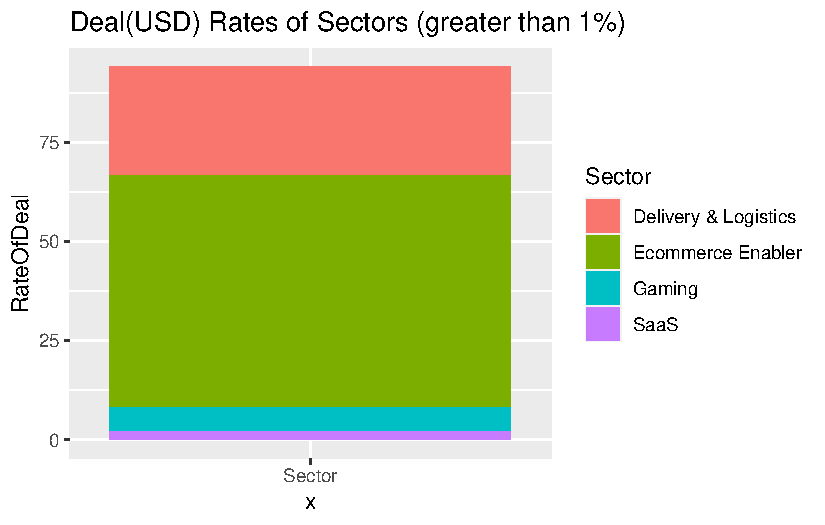
\includegraphics{./assignment1_files/figure-pdf/unnamed-chunk-5-1.pdf}

}

\end{figure}

\hypertarget{deal-amounts-who-makes-the-difference}{%
\subsubsection{Deal Amounts: Who makes the
difference?}\label{deal-amounts-who-makes-the-difference}}

\begin{Shaded}
\begin{Highlighting}[]
\NormalTok{df }\OtherTok{\textless{}{-}}\NormalTok{  data }\SpecialCharTok{\%\textgreater{}\%}
  \FunctionTok{group\_by}\NormalTok{(Company,Sector) }\SpecialCharTok{\%\textgreater{}\%}
  \FunctionTok{summarise}\NormalTok{(}\AttributeTok{Total=}\FunctionTok{n}\NormalTok{(),}\AttributeTok{TotalDealValue=}\FunctionTok{sum}\NormalTok{(DealValue))  }\SpecialCharTok{\%\textgreater{}\%}
  \FunctionTok{arrange}\NormalTok{(}\FunctionTok{desc}\NormalTok{(TotalDealValue))}

\FunctionTok{ggplot}\NormalTok{(df) }\SpecialCharTok{+}
  \FunctionTok{aes}\NormalTok{(}\AttributeTok{x =} \StringTok{""}\NormalTok{, }\AttributeTok{y =} \FunctionTok{log}\NormalTok{(TotalDealValue)) }\SpecialCharTok{+}
  \FunctionTok{geom\_boxplot}\NormalTok{(}\AttributeTok{fill =} \StringTok{"\#0c4c8a"}\NormalTok{) }\SpecialCharTok{+}
  \FunctionTok{theme\_minimal}\NormalTok{()}
\end{Highlighting}
\end{Shaded}

\begin{figure}[H]

{\centering 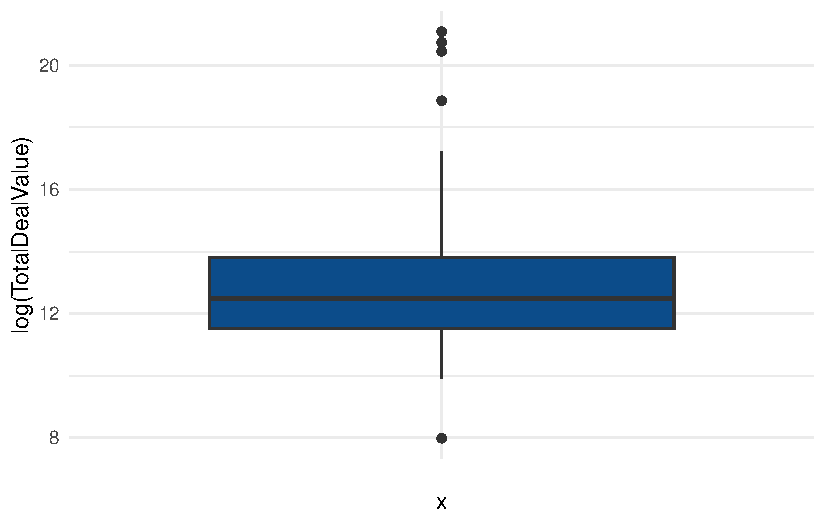
\includegraphics{./assignment1_files/figure-pdf/unnamed-chunk-6-1.pdf}

}

\end{figure}

\textbf{Which companies make the difference?}

\begin{Shaded}
\begin{Highlighting}[]
\NormalTok{lower\_bound }\OtherTok{\textless{}{-}} \FunctionTok{quantile}\NormalTok{(df}\SpecialCharTok{$}\NormalTok{TotalDealValue, }\FloatTok{0.01}\NormalTok{,}\AttributeTok{na.rm =} \ConstantTok{TRUE}\NormalTok{)}
\NormalTok{upper\_bound }\OtherTok{\textless{}{-}} \FunctionTok{quantile}\NormalTok{(df}\SpecialCharTok{$}\NormalTok{TotalDealValue, }\FloatTok{0.99}\NormalTok{,}\AttributeTok{na.rm =} \ConstantTok{TRUE}\NormalTok{)}

\NormalTok{upper\_outlier\_ind }\OtherTok{\textless{}{-}} \FunctionTok{which}\NormalTok{(df}\SpecialCharTok{$}\NormalTok{TotalDealValue }\SpecialCharTok{\textgreater{}}\NormalTok{ upper\_bound)}


\NormalTok{knitr}\SpecialCharTok{::}\FunctionTok{kable}\NormalTok{(df[upper\_outlier\_ind, ],}\AttributeTok{caption =} \StringTok{"Companies Making Difference"}\NormalTok{)}
\end{Highlighting}
\end{Shaded}

\begin{longtable}[]{@{}llrr@{}}
\caption{Companies Making Difference}\tabularnewline
\toprule()
Company & Sector & Total & TotalDealValue \\
\midrule()
\endfirsthead
\toprule()
Company & Sector & Total & TotalDealValue \\
\midrule()
\endhead
trendyol & Ecommerce Enabler & 1 & 1435000000 \\
Getir & Delivery \& Logistics & 4 & 1018000000 \\
hepsiburada & Ecommerce Enabler & 1 & 761481000 \\
\bottomrule()
\end{longtable}

\hypertarget{investors}{%
\subsubsection{Investors}\label{investors}}

\textbf{Investor Numbers by Sectors}

\begin{Shaded}
\begin{Highlighting}[]
\NormalTok{data\_investor }\OtherTok{\textless{}{-}} \FunctionTok{mutate}\NormalTok{(data,}
       \AttributeTok{investor\_number =} \FunctionTok{sapply}\NormalTok{(}\FunctionTok{strsplit}\NormalTok{(}\FunctionTok{as.character}\NormalTok{(data}\SpecialCharTok{$}\NormalTok{Investor), }\StringTok{","}\NormalTok{), length))}

\NormalTok{investor\_gg }\OtherTok{\textless{}{-}}\NormalTok{ data\_investor }\SpecialCharTok{\%\textgreater{}\%}
  \FunctionTok{group\_by}\NormalTok{(Sector) }\SpecialCharTok{\%\textgreater{}\%}
  \FunctionTok{summarise}\NormalTok{(}\AttributeTok{TotalNumberInvestor=}\FunctionTok{sum}\NormalTok{(investor\_number))  }\SpecialCharTok{\%\textgreater{}\%}
  \FunctionTok{arrange}\NormalTok{(}\FunctionTok{desc}\NormalTok{(TotalNumberInvestor)) }\SpecialCharTok{\%\textgreater{}\%}
  \FunctionTok{slice\_max}\NormalTok{(TotalNumberInvestor,}\AttributeTok{n=}\DecValTok{10}\NormalTok{)}

\FunctionTok{ggplot}\NormalTok{(}\AttributeTok{data=}\NormalTok{investor\_gg, }\FunctionTok{aes}\NormalTok{(}\AttributeTok{x=}\NormalTok{Sector, }\AttributeTok{y=}\NormalTok{TotalNumberInvestor)) }\SpecialCharTok{+}
  \FunctionTok{geom\_bar}\NormalTok{(}\AttributeTok{position=}\StringTok{"dodge"}\NormalTok{,}\AttributeTok{stat=}\StringTok{"identity"}\NormalTok{) }\SpecialCharTok{+} 
  \FunctionTok{ggtitle}\NormalTok{(}\StringTok{"Number of Investors by Sectors"}\NormalTok{) }\SpecialCharTok{+}
  \FunctionTok{theme}\NormalTok{(}\AttributeTok{axis.text.x =} \FunctionTok{element\_text}\NormalTok{(}\AttributeTok{angle =} \DecValTok{90}\NormalTok{))}
\end{Highlighting}
\end{Shaded}

\begin{figure}[H]

{\centering 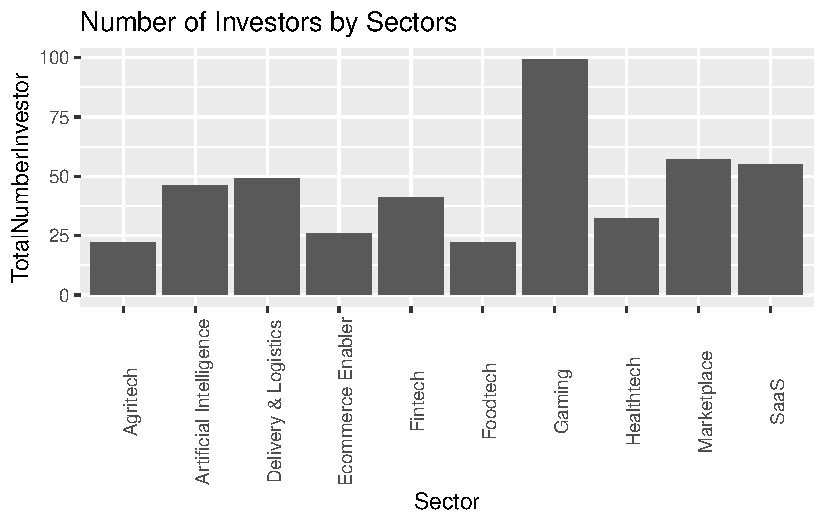
\includegraphics{./assignment1_files/figure-pdf/unnamed-chunk-8-1.pdf}

}

\end{figure}

\textbf{Investor Numbers by Origins : Most Multi-cultural Sector :
Agritech }

\begin{Shaded}
\begin{Highlighting}[]
\NormalTok{data\_inv\_origin }\OtherTok{\textless{}{-}} \FunctionTok{mutate}\NormalTok{(data,}
       \AttributeTok{origin\_number =} \FunctionTok{sapply}\NormalTok{(}\FunctionTok{strsplit}\NormalTok{(}\FunctionTok{as.character}\NormalTok{(data}\SpecialCharTok{$}\NormalTok{Origin), }\StringTok{","}\NormalTok{), length)) }

\NormalTok{inv\_or\_sec }\OtherTok{\textless{}{-}}\NormalTok{ data\_inv\_origin }\SpecialCharTok{\%\textgreater{}\%}
  \FunctionTok{group\_by}\NormalTok{(Sector) }\SpecialCharTok{\%\textgreater{}\%}
  \FunctionTok{summarise}\NormalTok{(}\AttributeTok{MaxOriginNumber =} \FunctionTok{max}\NormalTok{(origin\_number),}\AttributeTok{MeanOriginNumber =} \FunctionTok{mean}\NormalTok{(origin\_number)) }\SpecialCharTok{\%\textgreater{}\%}
  \FunctionTok{filter}\NormalTok{(MaxOriginNumber}\SpecialCharTok{\textgreater{}}\DecValTok{1}\NormalTok{) }\SpecialCharTok{\%\textgreater{}\%}
  \FunctionTok{arrange}\NormalTok{(}\FunctionTok{desc}\NormalTok{(MaxOriginNumber)) }\SpecialCharTok{\%\textgreater{}\%}
  \FunctionTok{top\_n}\NormalTok{(}\DecValTok{5}\NormalTok{)}
\end{Highlighting}
\end{Shaded}

\begin{verbatim}
Selecting by MeanOriginNumber
\end{verbatim}

\begin{Shaded}
\begin{Highlighting}[]
\NormalTok{knitr}\SpecialCharTok{::}\FunctionTok{kable}\NormalTok{(inv\_or\_sec)}
\end{Highlighting}
\end{Shaded}

\begin{longtable}[]{@{}lrr@{}}
\toprule()
Sector & MaxOriginNumber & MeanOriginNumber \\
\midrule()
\endhead
Agritech & 5 & 1.625000 \\
Ecommerce Enabler & 4 & 1.666667 \\
Delivery \& Logistics & 3 & 1.307692 \\
Advertising & 2 & 1.500000 \\
Foodtech & 2 & 1.222222 \\
\bottomrule()
\end{longtable}

\textbf{Investors: Financial or Non-Financial?}

\begin{Shaded}
\begin{Highlighting}[]
\NormalTok{df1 }\OtherTok{\textless{}{-}}\NormalTok{ data }\SpecialCharTok{\%\textgreater{}\%}
  \FunctionTok{group\_by}\NormalTok{(Sector) }\SpecialCharTok{\%\textgreater{}\%}
  \FunctionTok{summarise}\NormalTok{(}
    \AttributeTok{Total =} \FunctionTok{n}\NormalTok{(),}
    \AttributeTok{Financial =} \FunctionTok{sum}\NormalTok{(Financial }\SpecialCharTok{==} \StringTok{"Yes"}\NormalTok{)}
\NormalTok{  ) }\SpecialCharTok{\%\textgreater{}\%}
  \FunctionTok{mutate}\NormalTok{(}\AttributeTok{FinancialInvestorPercentage =}\NormalTok{(Financial}\SpecialCharTok{/}\NormalTok{Total)}\SpecialCharTok{*}\DecValTok{100}\NormalTok{ ) }\SpecialCharTok{\%\textgreater{}\%}
  \FunctionTok{filter}\NormalTok{(Total}\SpecialCharTok{\textgreater{}}\DecValTok{1}\NormalTok{) }\SpecialCharTok{\%\textgreater{}\%}
  \FunctionTok{arrange}\NormalTok{(}\FunctionTok{desc}\NormalTok{(Financial),}\FunctionTok{desc}\NormalTok{(FinancialInvestorPercentage))}

\NormalTok{knitr}\SpecialCharTok{::}\FunctionTok{kable}\NormalTok{(}\FunctionTok{head}\NormalTok{(df1,}\DecValTok{10}\NormalTok{))}
\end{Highlighting}
\end{Shaded}

\begin{longtable}[]{@{}
  >{\raggedright\arraybackslash}p{(\columnwidth - 6\tabcolsep) * \real{0.3529}}
  >{\raggedleft\arraybackslash}p{(\columnwidth - 6\tabcolsep) * \real{0.0882}}
  >{\raggedleft\arraybackslash}p{(\columnwidth - 6\tabcolsep) * \real{0.1471}}
  >{\raggedleft\arraybackslash}p{(\columnwidth - 6\tabcolsep) * \real{0.4118}}@{}}
\toprule()
\begin{minipage}[b]{\linewidth}\raggedright
Sector
\end{minipage} & \begin{minipage}[b]{\linewidth}\raggedleft
Total
\end{minipage} & \begin{minipage}[b]{\linewidth}\raggedleft
Financial
\end{minipage} & \begin{minipage}[b]{\linewidth}\raggedleft
FinancialInvestorPercentage
\end{minipage} \\
\midrule()
\endhead
Gaming & 51 & 27 & 52.94118 \\
SaaS & 28 & 19 & 67.85714 \\
Fintech & 23 & 17 & 73.91304 \\
Delivery \& Logistics & 13 & 11 & 84.61538 \\
Healthtech & 14 & 11 & 78.57143 \\
Marketplace & 17 & 11 & 64.70588 \\
Artificial Intelligence & 14 & 9 & 64.28571 \\
Ecommerce Enabler & 9 & 7 & 77.77778 \\
Foodtech & 9 & 7 & 77.77778 \\
Biotech & 6 & 6 & 100.00000 \\
\bottomrule()
\end{longtable}

\hypertarget{when-the-investments-take-place-most}{%
\subsubsection{When the investments take place
most?}\label{when-the-investments-take-place-most}}

\begin{Shaded}
\begin{Highlighting}[]
\NormalTok{df }\OtherTok{\textless{}{-}}\NormalTok{  data }\SpecialCharTok{\%\textgreater{}\%}
  \FunctionTok{mutate}\NormalTok{(}\AttributeTok{Month =} \FunctionTok{month}\NormalTok{(data}\SpecialCharTok{$}\NormalTok{Date, }\AttributeTok{label=}\ConstantTok{TRUE}\NormalTok{)) }\SpecialCharTok{\%\textgreater{}\%}
  \FunctionTok{mutate}\NormalTok{(}\AttributeTok{Quarter =} \FunctionTok{paste}\NormalTok{(}\StringTok{"2021 Q"}\NormalTok{, }\FunctionTok{quarter}\NormalTok{(data}\SpecialCharTok{$}\NormalTok{Date)))  }\SpecialCharTok{\%\textgreater{}\%}
  \FunctionTok{group\_by}\NormalTok{(Quarter) }\SpecialCharTok{\%\textgreater{}\%}
  \FunctionTok{summarise}\NormalTok{(}\AttributeTok{Total=}\FunctionTok{n}\NormalTok{())}\SpecialCharTok{\%\textgreater{}\%}
  \FunctionTok{arrange}\NormalTok{(Quarter) }

\FunctionTok{ggplot}\NormalTok{(}\AttributeTok{data=}\NormalTok{df, }\FunctionTok{aes}\NormalTok{(}\AttributeTok{x=}\NormalTok{Quarter, }\AttributeTok{y=}\NormalTok{Total, }\AttributeTok{group=}\DecValTok{1}\NormalTok{)) }\SpecialCharTok{+}
  \FunctionTok{geom\_line}\NormalTok{()}\SpecialCharTok{+}
  \FunctionTok{geom\_point}\NormalTok{() }\SpecialCharTok{+}
  \FunctionTok{ylim}\NormalTok{(}\DecValTok{0}\NormalTok{,}\DecValTok{100}\NormalTok{) }\SpecialCharTok{+}
  \FunctionTok{ggtitle}\NormalTok{(}\StringTok{"Number of Investments Quarters {-} 2021"}\NormalTok{)}
\end{Highlighting}
\end{Shaded}

\begin{figure}[H]

{\centering 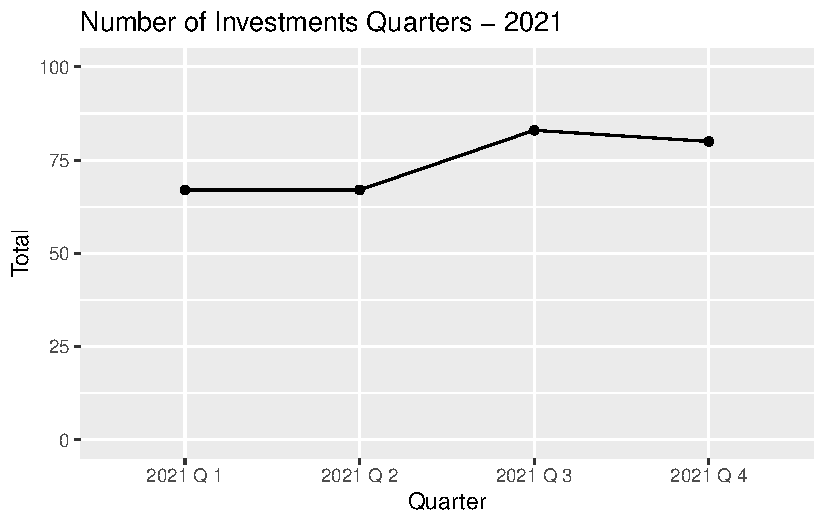
\includegraphics{./assignment1_files/figure-pdf/unnamed-chunk-11-1.pdf}

}

\end{figure}

\begin{Shaded}
\begin{Highlighting}[]
\NormalTok{df1 }\OtherTok{\textless{}{-}}\NormalTok{  data }\SpecialCharTok{\%\textgreater{}\%}
  \FunctionTok{mutate}\NormalTok{(}\AttributeTok{Month =} \FunctionTok{month}\NormalTok{(data}\SpecialCharTok{$}\NormalTok{Date, }\AttributeTok{label=}\ConstantTok{TRUE}\NormalTok{)) }\SpecialCharTok{\%\textgreater{}\%}
  \FunctionTok{group\_by}\NormalTok{(Month) }\SpecialCharTok{\%\textgreater{}\%}
  \FunctionTok{summarise}\NormalTok{(}\AttributeTok{Total=}\FunctionTok{n}\NormalTok{())}\SpecialCharTok{\%\textgreater{}\%}
  \FunctionTok{arrange}\NormalTok{(Month) }

\FunctionTok{ggplot}\NormalTok{(}\AttributeTok{data=}\NormalTok{df1, }\FunctionTok{aes}\NormalTok{(}\AttributeTok{x=}\NormalTok{Month, }\AttributeTok{y=}\NormalTok{Total, }\AttributeTok{group=}\DecValTok{1}\NormalTok{)) }\SpecialCharTok{+}
  \FunctionTok{geom\_line}\NormalTok{()}\SpecialCharTok{+}
  \FunctionTok{geom\_point}\NormalTok{() }\SpecialCharTok{+}
  \FunctionTok{ylim}\NormalTok{(}\DecValTok{0}\NormalTok{,}\DecValTok{100}\NormalTok{) }\SpecialCharTok{+}
  \FunctionTok{ggtitle}\NormalTok{(}\StringTok{"Number of Investments Monthly {-} 2021"}\NormalTok{)}
\end{Highlighting}
\end{Shaded}

\begin{figure}[H]

{\centering 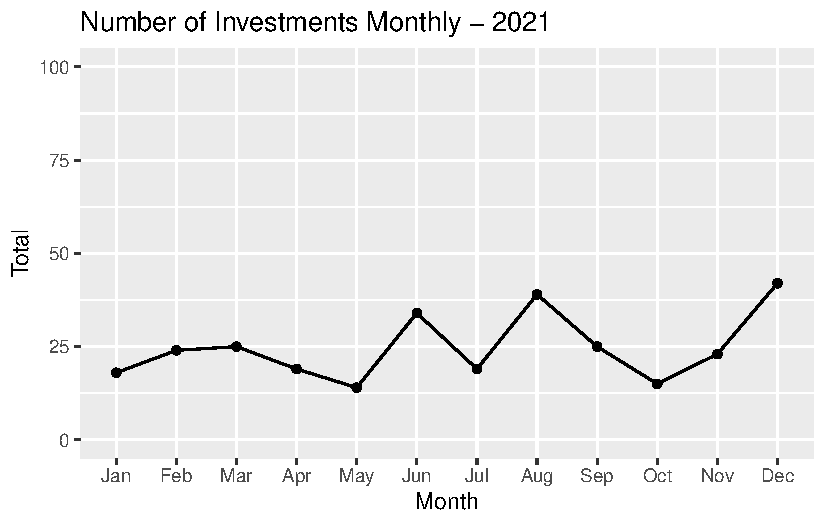
\includegraphics{./assignment1_files/figure-pdf/unnamed-chunk-12-1.pdf}

}

\end{figure}

\#We can say that Non-financial investors mostly invested in Acquisiton
Stage

\begin{Shaded}
\begin{Highlighting}[]
  \FunctionTok{ggplot}\NormalTok{(data,}\FunctionTok{aes}\NormalTok{(}\AttributeTok{x =}\NormalTok{ Stage, }\AttributeTok{y=}\NormalTok{Sector, }\AttributeTok{fill =}\NormalTok{ Financial)) }\SpecialCharTok{+}
    \FunctionTok{geom\_dotplot}\NormalTok{(}\AttributeTok{binaxis =} \StringTok{"y"}\NormalTok{, }\AttributeTok{stackdir =} \StringTok{"center"}\NormalTok{)}
\end{Highlighting}
\end{Shaded}

\begin{verbatim}
Bin width defaults to 1/30 of the range of the data. Pick better value with `binwidth`.
\end{verbatim}

\begin{figure}[H]

{\centering 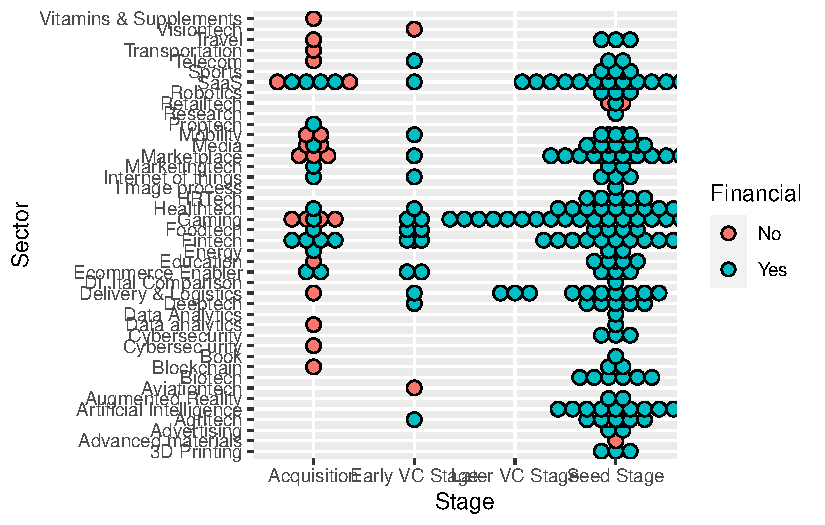
\includegraphics{./assignment1_files/figure-pdf/unnamed-chunk-13-1.pdf}

}

\end{figure}



\end{document}
